\documentclass{emulateapj}
%\documentclass[12pt,preprint]{aastex}

\usepackage[utf8]{inputenc}
\usepackage{graphicx}
\usepackage{float}
\usepackage{amsmath}
\usepackage{epsfig,floatflt}
\usepackage{url}
\setcitestyle{square}

\begin{document}

\title{Project 4}

\author{Stig-Nicolai Foyn}

\email{stignicf@student.matnat.uio.no}

\altaffiltext{1}{Institute of Physics, University of
  Oslo, P.O.\ Box 1029 Blindern, N-0315 Oslo, Norway}

%\date{Received - / Accepted -}

\begin{abstract}
In this study of phase transitions of magnetic systems, we study the Ising model by using Monte Carlo simulation on a binary magnetic spin state lattice. The algorithm used is the metropolis algorithm (called a Markov Chain Monte Carlo method). To benchmar our program we analytically solve the problem for a $2x2$ lattice and find that our numerical results are reasonably close. We then move on to a larger system ($L=20$) to test the equillibration time and to study the probability distribution of energies under two different temperatures. Our distribution for $T=1.0$ was almost entirely in the ground state energy, while we had an almost normal distribution for $T=2.4$. For even larger lattices $L=140$ we study the expectation values of mean magnetic moment, energy, heat capacity and susceptibility. We use this to conclude with our transformation being a second order transformation from a ferromagnetic (high magnetization) to a paramagnetic material (almost zero magnetization). Lastly we use the susceptibility to study the critical temperature of the lattice found to be $T_C=2.263$ as compared to the analytical $T_C = 2.269$.
\end{abstract}

\keywords{Ising model --- computational science --- methods: Monte Carlo, Metropolis Algorithm}

\section{Introduction}
\label{sec:introduction}
This is a study of the Ising model in two dimensions, focusing on utilizing Monte Carlo simulation with the Metropolis algorithm to simulate binary spin states in a lattice with periodic boundary conditions. The different spin-orientations have a set of predictable energies, and the algorithm decides whether a spin should be flipped or not, with a bias towards the equilibrium energy. The Ising model describes phase transitions of magnetic systems without external fields and is characterized by the expression.
%
\begin{equation*}
    E = -J \sum_{kl}^{N} s_{k}s_{l}
\end{equation*}
%
When calculating statistical physics the Boltzmann distribution, used for the macrostates of a system in the canonical ensemble. This states that the probability of a system being in a state s is given by.
\begin{equation*}
    P(E) = \frac{1}{Z} e^{-\beta E_s}
\end{equation*}
%
Where $E_s$ is the energy in state s, and $Z$ is the partition function given by.
%
\begin{equation*}
    Z(\beta) = \sum_s e^{-\beta E_s}
\end{equation*}
%
The motivation behind using the Metropolis algorithm is the fact that it only considers the ratio between probabilities. When using the Ising model in two dimentions the partition function has $2^N$ configurations where $N = LxL$. This means that for a $L = 20$ lattice we would have $2^400$ configurations, which is completely unreasonable to calculate, even with a supercomputer. So being able to ignore the partition function means that we can, with relative ease, approximate the characteristics of much larger lattices.

%(Demonstrate usefulness of object-oriented code)

\section{Theory and method}
\label{sec:method}

\subsection{Ising model}
%
Because the lattice is of finite size we risk having effects from the borders affect our results. However one way to approximate infinite lattices is by letting the spin states on the borders loop around and be equal to each other, called periodic boundary conditions.
%
For the $L=2$ spin lattice using the Ising model we have analytical values. Deriving these will serve as a benefit when benchmarking the precision of the metropolis algorithm. In table \ref{tab:results1} (found in \cite{bib:project4}) we can see the energies and degeneracy of the energies for the $2x2$ lattice, from this we can derive the partition function and then the mean energy.
%
\begin{deluxetable}{lccc}
%\tablewidth{0pt}
\tablecaption{\label{tab:results1}}
\tablecomments{All states for a 2x2 lattice, with corresponding energies and magnetic moment. While the system is in the ground state all spins point in the same direction.}
\tablecolumns{4}
\tablehead{Spins up & Degeneracy & Energy & Magnetic moment }
\startdata
4 & 1 & -8J & 4 \\
3 & 4 & 0 & 2 \\
2 & 4 & 0 & 0 \\
2 & 2 & 8J & 0 \\
1 & 4 & 0 & -2 \\
0 & 1 & -8J & -4 \\
\enddata
\end{deluxetable}
%


%
\begin{equation*}
    Z = \sum_{ \text{All microstates}} e^{-\beta E_{i}} = 2e^{8\beta J} + 12e^{0} + 2e^{-8\beta J}
\end{equation*}
%
Using this identity for $\cosh(x)$:
%
\begin{equation*}
    \cosh(x) = \frac{1}{2} (e^{-x} + e^{x})
\end{equation*}
%
The identity is inserted to the expression found for the partition function:
%
\begin{align*}
    \langle E \rangle &= \frac{\delta ln(Z)}{\delta \beta} = \frac{1}{Z}\frac{\delta Z}{\delta \beta}\\
    &= \frac{1}{Z}\frac{\delta }{\delta \beta} (12 + 4 \cosh(8\beta J))\\
    &= \frac{8 J \sinh({8 \beta J})}{3 +  \cosh({8\beta J})}\\
\end{align*}
%
The heat capacity can now be derived by using the expression below:
%
\begin{align*}
    C_{V} &= \frac{1}{kT^2} \frac{\delta^2 ln(Z)}{\delta \beta^2} = \frac{1}{kT^2} \frac{\delta}{\delta \beta}(\frac{\delta ln(Z)}{\delta \beta})
    = \frac{1}{kT^2} \frac{\delta}{\delta \beta}(\langle E \rangle)\\
    &= \frac{1}{kT^2}\frac{(64 J^2 \cosh({8 \beta J}))(3 + \cosh (8 \beta J)) - 64 J^2 \sinh({8 \beta J}^2)}{(3 + \cosh (8 \beta J))^2}.\\
\end{align*}
%
Magnetization is derived from this expression:
%
\begin{align*}
    \langle |M| \rangle &= \frac{1}{Z} \sum_{i} (M_{i})e^{\beta J E_{i}} \\
    &= \frac{1}{Z}(|4|e^{8\beta J} + 4|2|e^{0} + 0 + 0 + 4|-2|e^{0} + |-4|e^{8\beta J}) \\
    &= \frac{2e^{8\beta J}+4}{3 + \cosh(8\beta J)} \\
\end{align*}
%
And using the expression found for magnetization the susceptibility can be derived as below:
%
\begin{align*}
    \langle M^2 \rangle &= \frac{1}{Z} \sum_{i} (M_{i})e^{\beta J E_{i}} \\
    &= \frac{1}{Z} (2 \times 16e^{8\beta J} + 2 \times 16e^{0}) \\
    \chi &= \frac{1}{kT}\langle M^2 \rangle = \frac {1}{kT} \frac{8e^{8\beta J} + 8}{3+\cosh(8\beta J)}\\
\end{align*}

%
The numerical results when using the analytical the algorithm
%
%
\subsection{Monte Carlo simulation}
As previously mentioned we draw a clear benefit from the fact that the Metropolis algorithm only considers the ratio between the probabilities of finding the system in a certain state. The probabilities of changing state, or in our case the probability of flipping a spin is given by:
%
\begin{equation*}
    P_{flip} = \frac{P_{i}}{P_{j}} = \frac{(1/Z)e^{-\beta E_i}}{(1/Z)e^{-\beta E_j}} = \frac{e^{-\beta E_i}}{e^{-\beta E_j}} = e^{\beta \Delta E}
\end{equation*}
%
Since the partition function is the same for the entire system we can remove it entirely. When implementing the metropolis algorithm we implement this as a test, to check if we should accept or reject the change of state. A random number $rng \in [0,1]$ will is selected, if this number exceeds the probability of changing state then we accept the flip of spin:
%
\begin{equation*}
    rng \leq e^{\beta \Delta E}
\end{equation*}
%
If this condition however is not met, the lattice keeps its old configuration and we move on to test the next possible change of spin. As spin states are accepted or rejected we update our expectation values. When it comes to the change in energy we are fortunate as there is only 5 different possible values for $\Delta E$ as exemplified below:
%
\begin{equation*}
    E = -4J
    \begin{bmatrix}
        & \uparrow &  \\
        \uparrow & \uparrow & \uparrow \\
         & \uparrow &
    \end{bmatrix}
    =>
    E = 4J
    \begin{bmatrix}
        & \uparrow &  \\
        \uparrow & \downarrow & \uparrow \\
         & \uparrow &
    \end{bmatrix}
\end{equation*}
%
%
\begin{equation*}
    E = -2J
    \begin{bmatrix}
        & \uparrow &  \\
        \downarrow & \uparrow & \uparrow \\
         & \uparrow &
    \end{bmatrix}
    =>
    E = 2J
    \begin{bmatrix}
        & \uparrow &  \\
        \downarrow & \downarrow & \uparrow \\
         & \uparrow &
    \end{bmatrix}
\end{equation*}
%
%
\begin{equation*}
    E = 0J
    \begin{bmatrix}
        & \uparrow &  \\
        \downarrow & \uparrow & \uparrow \\
         & \downarrow &
    \end{bmatrix}
    =>
    E = 0J
    \begin{bmatrix}
        & \uparrow &  \\
        \downarrow & \downarrow & \uparrow \\
         & \downarrow &
    \end{bmatrix}
\end{equation*}
%
%
\begin{equation*}
    E = -2J
    \begin{bmatrix}
        & \downarrow &  \\
        \downarrow & \uparrow & \uparrow \\
         & \downarrow &
    \end{bmatrix}
    =>
    E = 2J
    \begin{bmatrix}
        & \downarrow &  \\
        \downarrow & \downarrow & \uparrow \\
         & \downarrow &
    \end{bmatrix}
\end{equation*}
%
%
\begin{equation*}
    E = -4J
    \begin{bmatrix}
        & \downarrow &  \\
        \downarrow & \uparrow & \downarrow \\
         & \downarrow &
    \end{bmatrix}
    =>
    E = 4J
    \begin{bmatrix}
        & \downarrow &  \\
        \downarrow & \downarrow & \downarrow \\
         & \downarrow &
    \end{bmatrix}
\end{equation*}
%
The energy differences are then as follows. The first state has $\Delta E = 8$ the second $\Delta E = 4$, the third $\Delta E = 0$, the fourth $\Delta E = -4$ and lastly the fifth $\Delta E = -8$. With these energies pre-calculated our program will run faster than if we were to flip all spins and then calculate the change in energy, which would have been unreasonably slow.
%
\subsection{Phase transitions}
%
Approaching critical temperature results in both heat capacity and susceptibility of our lattice approaching infinity, meaning that the peaks of our results serve as our approximation to critical temperature. The expressions for the aforementioned expectation values and the critical temperature scales as:
%
\begin{equation*}
    C_{V} \sim |T_{C}-T|^{-\alpha}
\end{equation*}
%
\begin{equation*}
    \chi \sim |T_{C}-T|^{-\nu}
\end{equation*}
%
\begin{equation*}
    T_{C}(L) T_{C}(L=\infty) \propto a L^{- 1 / \nu}
\end{equation*}
%
With $\nu = 1$ and $a$ and $\alpha$ both being positive constants we get, this value for the critical temperature:
%
\begin{equation*}
    T_{C}(L=\infty) \approx T_{C}(L) -\frac{1}{L}
\end{equation*}
%
\section{Results}
\label{sec:results}
%
To benchmark the Monte Carlo method analytical values for a $L = 2$ ($2x2$ spin) lattice are used.
%
\begin{deluxetable}{lccc}
%\tablewidth{0pt}
\tablecaption{\label{tab:results2}}
\tablecomments{Table comparing analytical and simulated values found for the L=2 lattice. The expectation values from the Monte Carlo model are found using $cycles = 10000$ on one CPU with no cutoff, and $cycles = 1e6$ divided up between 8 CPU threads (effective cycles per thread $cycles = 125000$) with a cutoff at $cycles = 10000$.}
\tablecolumns{3}
\tablehead{Parameter & Analytical & $cycles = 1e4$ & $cycles = 1e6$}
\startdata
$\langle E \rangle$ & -1.99598 & -1.9962 & -1.99609 \\
$\langle |M| \rangle$ & 0.998660  & 0.99865 & 0.998708 \\
$C_{V}$ & 0.03208233 & 0.0303422 & 0.0312116 \\
$\chi$ & 3.993303 & 3.9935 & 3.99351  \\
\enddata
\end{deluxetable}
%
%
\begin{figure}[H]
{{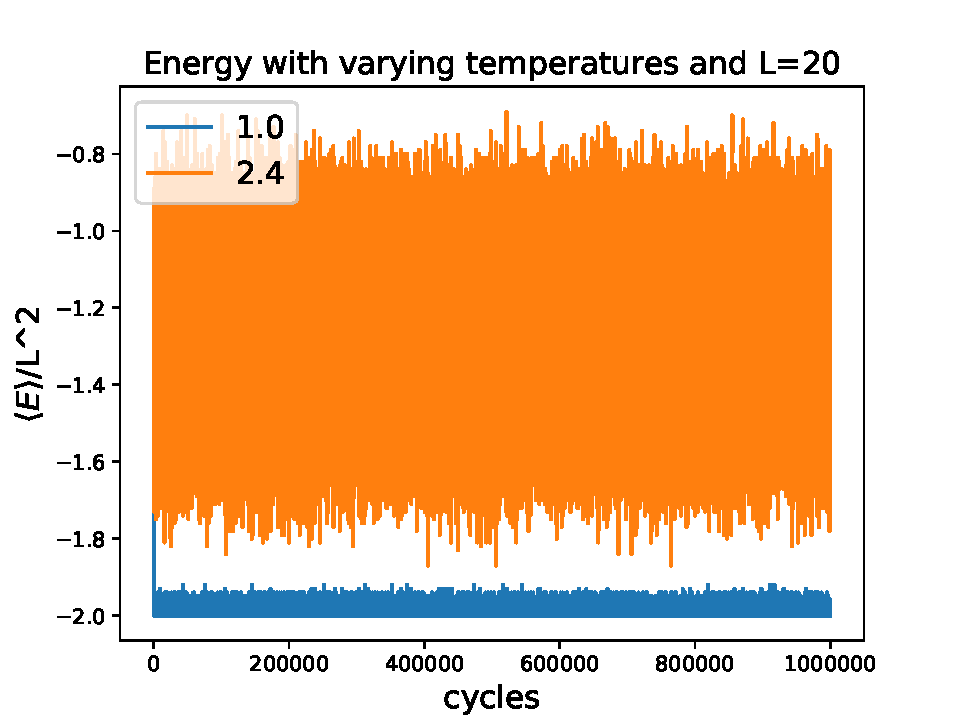
\includegraphics[scale=0.53]{DEL20_MC1M.pdf}}
\subfloat{(a) This plot shows the mean energy for a disordered lattice with temperatures $T=1.0$ and $T=2.4$ for $1e6$ cycles.}
}\qquad
{{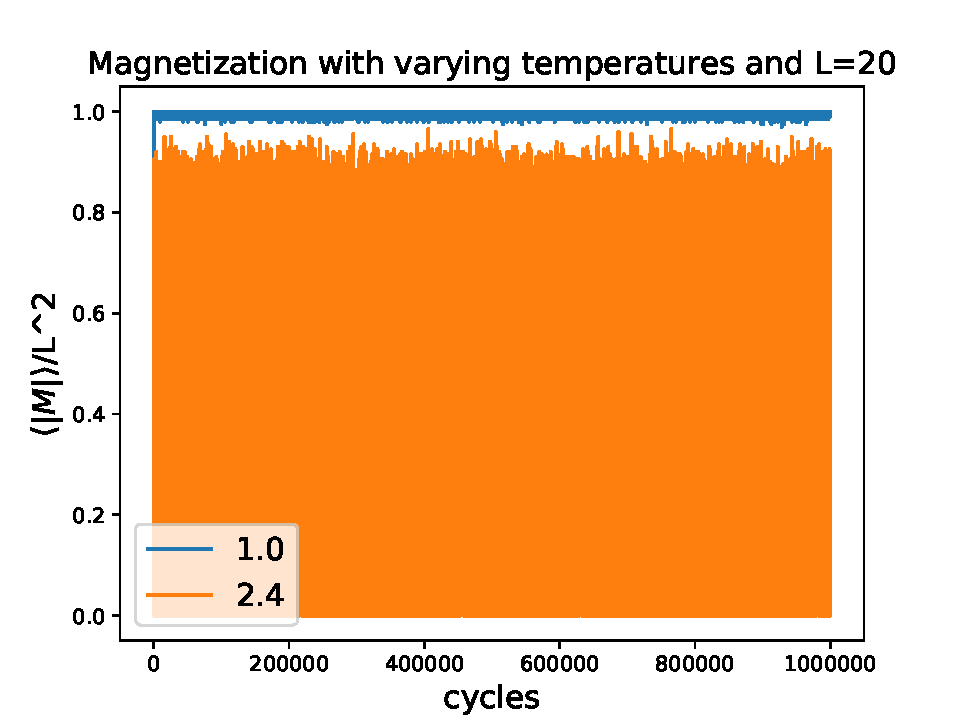
\includegraphics[scale=0.53]{DML20_MC1M.pdf}}
\subfloat{(b) This plot shows the mean magnetization for a disordered lattice with temperatures $T=1.0$ and $T=2.4$ for $1e6$ cycles.}
}\qquad
\caption{Plot for a $L=20$ lattice in ground state, the noise for higher temperatures (and energies) is significant, in addition while not visible in this plot the eqilibration time is definetly before $500$ cycles (seen in the next plot).}
\label{fig:Disordered}
\end{figure}
%
%
\begin{figure}[H]
{{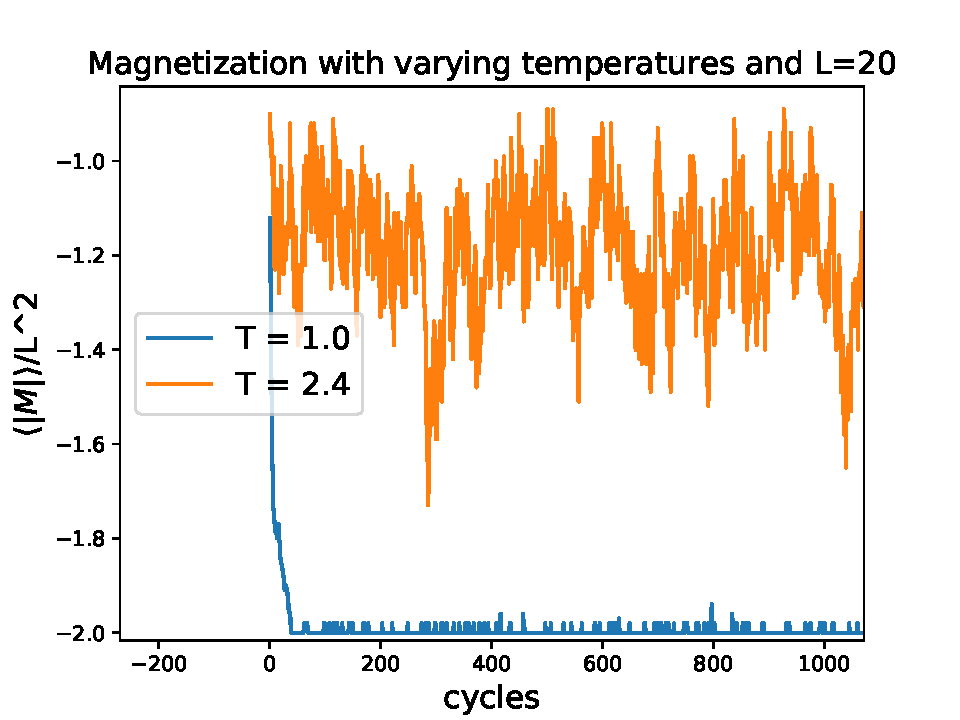
\includegraphics[scale=0.53]{zoomDEL20_MC1M.pdf}}
\subfloat{(a) This is a closeup of the mean energy in first few cycles from the disordered state plot \ref{fig:Disordered}}
}\qquad
{{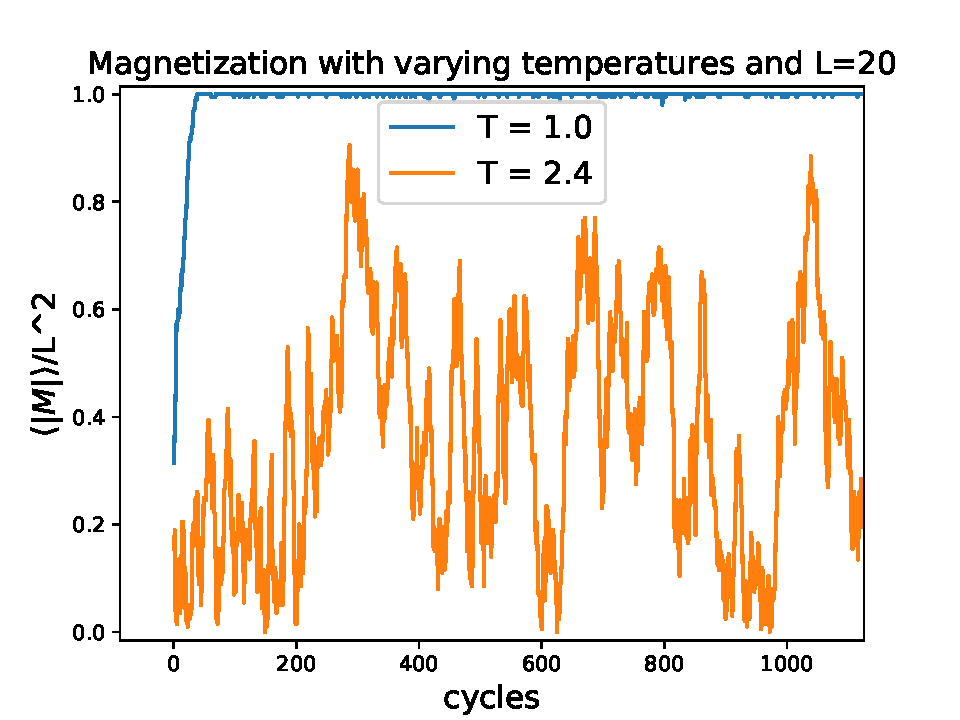
\includegraphics[scale=0.53]{zoomDML20_MC1M.pdf}}
\subfloat{(b) This is a closeup of the mean magnetic moment in the first few cycles from the disordered state plot \ref{fig:Disordered}}
}\qquad
\caption{This plot serves as visual aid for the comments made about equillibration time in fig.\ref{fig:Disordered}. The equillibration time is seemingly before $cycles = 100$ and as stated definitely before $cycles=500$.}
\label{fig:zoomOrdered}
\end{figure}
%

%
\begin{figure}[H]
{{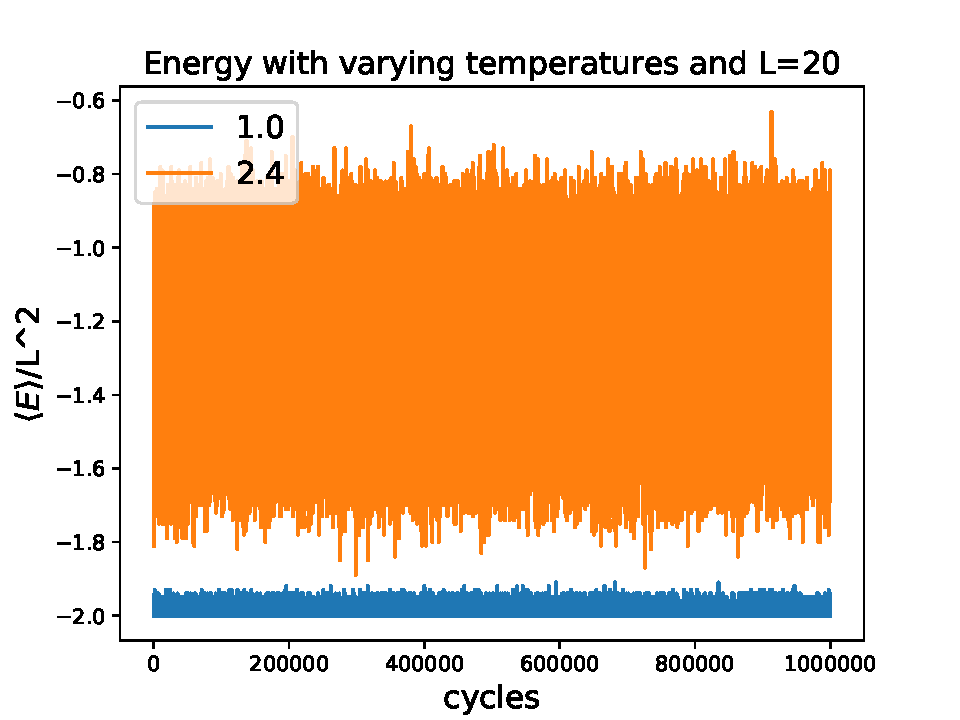
\includegraphics[scale=0.53]{OEL20_MC1M.pdf}}
\subfloat{(a) This plot is the energy for the ordered lattice case, with temperatures $T=1.0$ and $T = 2.4$, using $1e6$ cycles.}
}\qquad
{{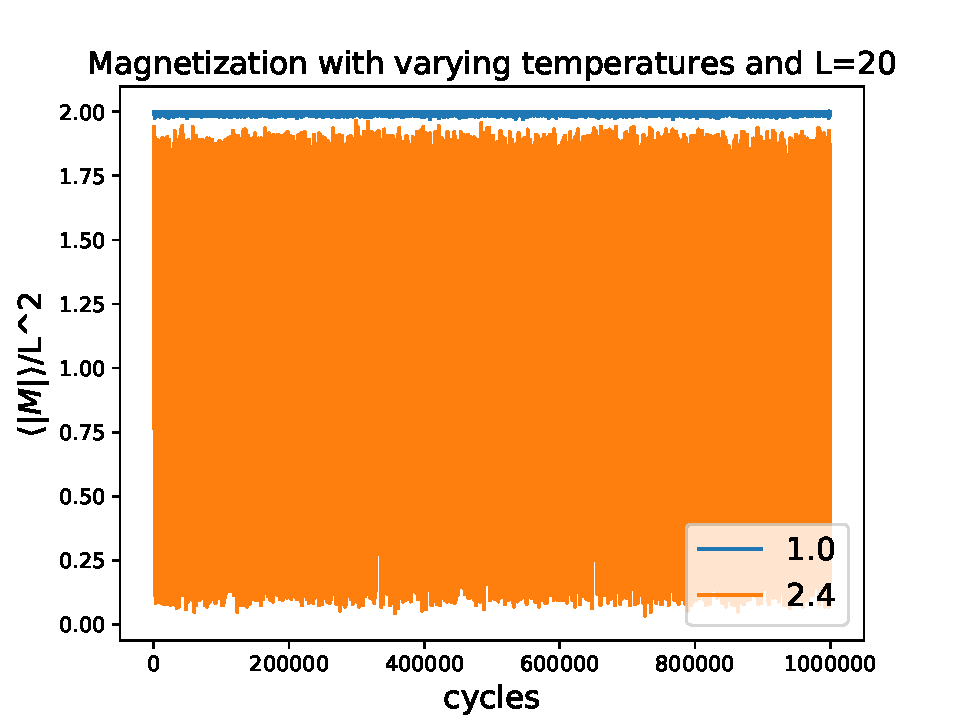
\includegraphics[scale=0.53]{OML20_MC1M.pdf}}
\subfloat{(b) This plot is mean magnetization for the ordered lattice case, for temperatures $T=1.0$ and $T = 2.4$, with $1e6$ cycles.}
}\qquad
\caption{Plot for a $L=20$ lattice in ground state, the most significant difference between this and the disordered lattice case is that the energy and magnetization starts in ground state. This in effect looks similar to having a cutoff value for the disordered state.}
\label{fig:Ordered}
\end{figure}
%
%
\begin{figure}[H]
{{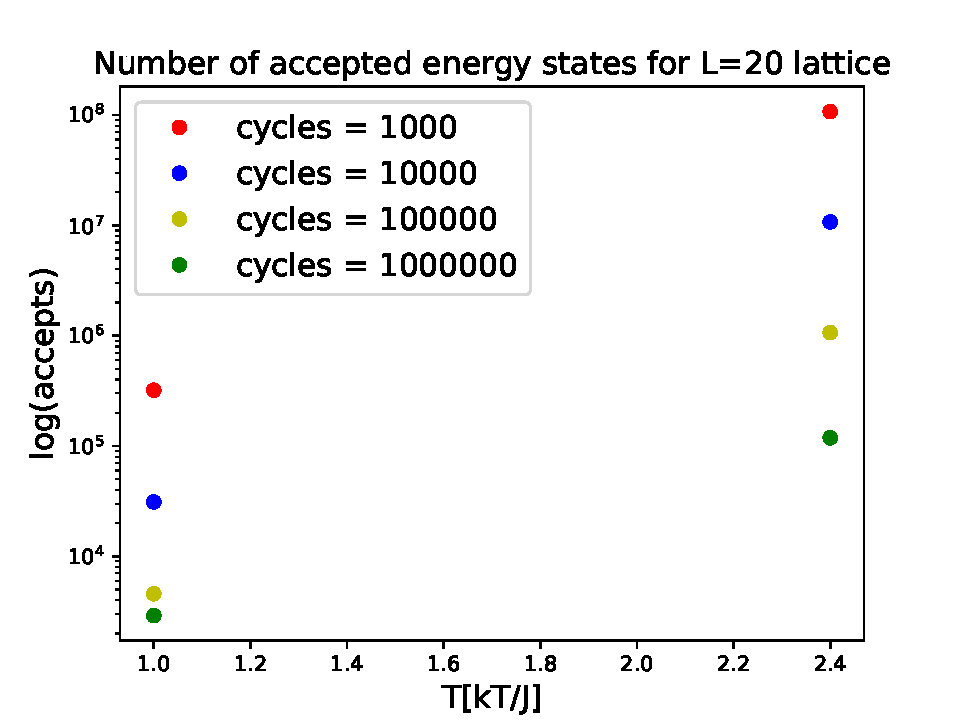
\includegraphics[scale=0.53]{acceptspercyc.pdf}}
\subfloat{(a) Number of accepted states at different amounts of cycles, at temperatures $T = 1.0$ and $T = 2.4$, the amount of cycles does not scale linearly with temperature.}
}\qquad
{{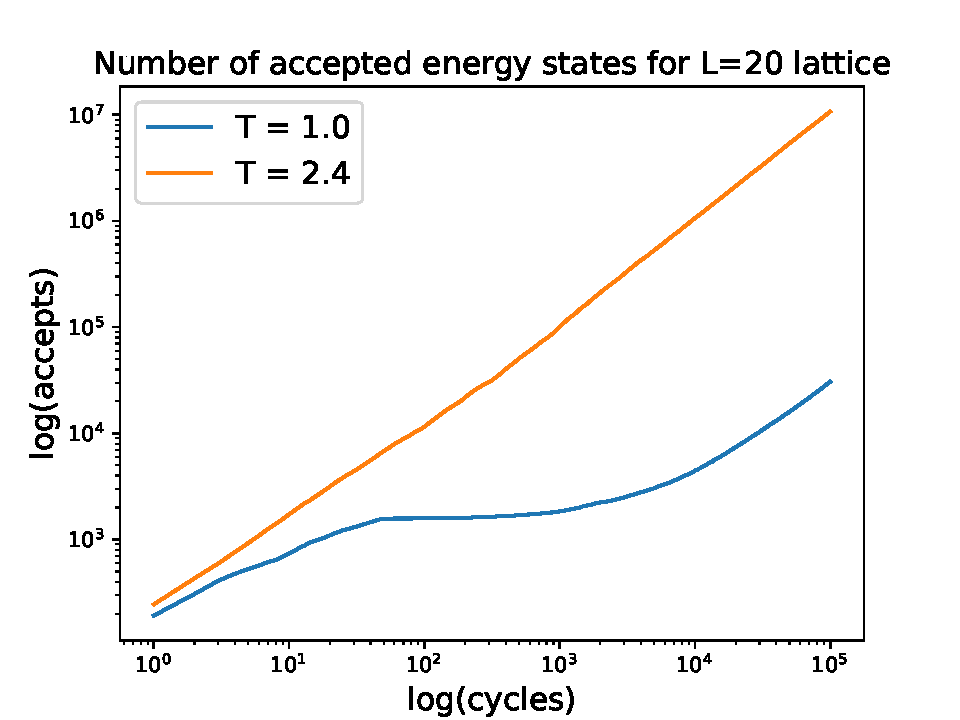
\includegraphics[scale=0.53]{accepts.pdf}}
\subfloat{(b) Number of accepted states as function of the amount of cycles, at temperatures $T = 1.0$ and $T = 2.4$, this to show the temperature dependency on the amount of cycles in a more comprehensive plot.}
}\qquad
\caption{Two different ways to show the amount of accepted energies as function of the amount of cycles and temperature, both run with a $L=20$ lattice.}
\label{fig:accepts}
\end{figure}
%
%
\begin{figure}[H]
{{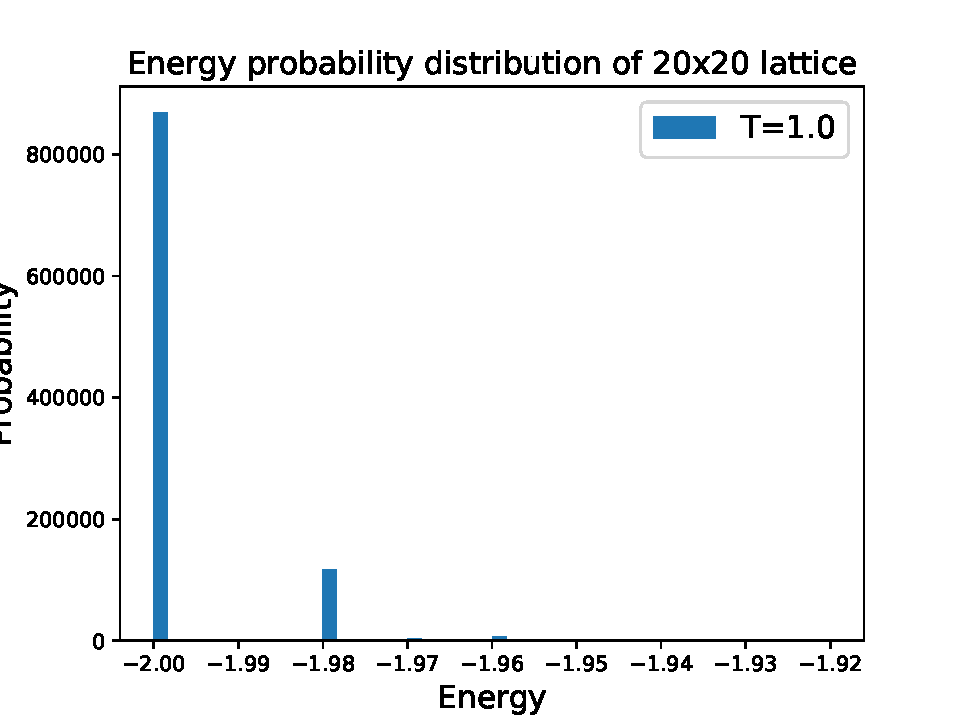
\includegraphics[scale=0.53]{ProbDistribution10_20x20.pdf}}
\subfloat{(a) This plot shows the distribution for temperature $T=1.0$, for low temperatures such as $T=1.0$ the energy distribution favours the ground state energy.}
}\qquad
{{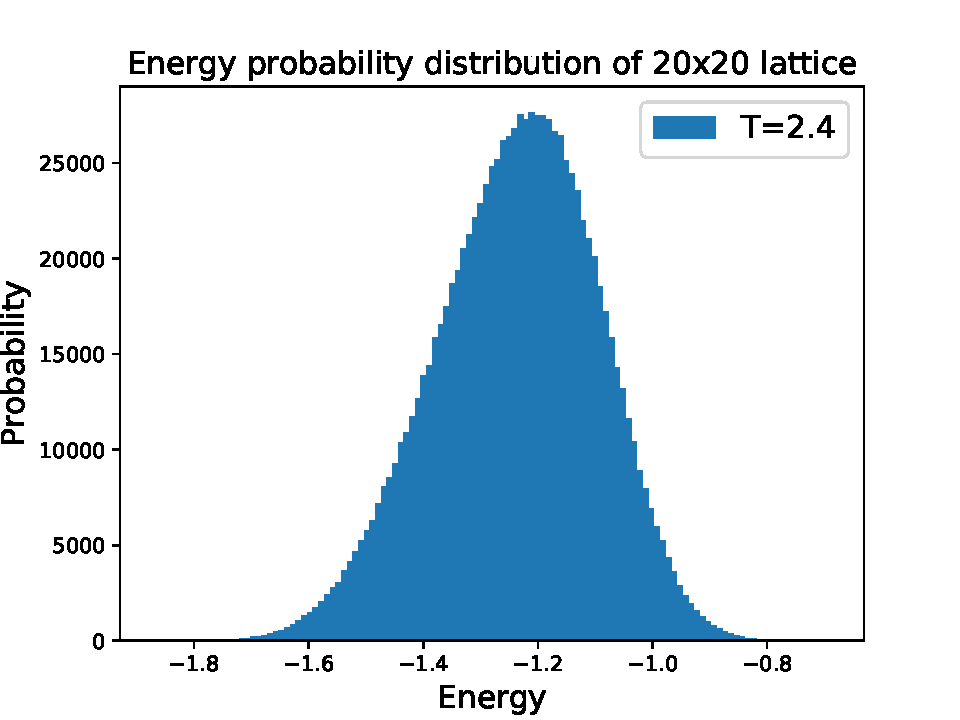
\includegraphics[scale=0.53]{ProbDistribution24_20x20.pdf}}
\subfloat{(b) This plot shows the distribution for temperature $T=2.4$, this looks like a slightly skewed normal probability distribution.}
}\qquad
\caption{This is the energy probability distribution for a $L=20$ lattice with $cycles=1e6$, these distribution histograms are not normalized.}
\label{fig:PD}
\end{figure}
%
Now that we have benchmarked our program and seen some results its time to test how fast it runs. Results of these tests are shown in table \ref{tab:results3}, where we compare CPU-time when using one thread and CPU-time using 8 threads. Table \ref{tab:results4} of CPU-times show the timing of the program based on lattice size.
\newline
\newline
%
\begin{deluxetable}{lccc}
%\tablewidth{0pt}
\tablecaption{\label{tab:results3}}
\tablecomments{Table displaying CPU-time running of the metropolis algorithm running on 1 core and 8 cores. This test was done on a $L=20$ lattice, with $cycles = 1e6$, temperature interval starting with $T_s = 2.2$ ending at $T_f = 2.5$ with temperature steps of $T_dt = 0.05$.}
\tablecolumns{3}
\tablehead{Nr of threads & 1 & 8}
\startdata
    CPU-time 1 & 89.253 & 19.285 \\
    CPU-time 2 & 88.088 & 19.872 \\
    CPU-time 3 & 88.823 & 18.703 \\
    Average & 88.722 & 19.287 \\
\enddata
\end{deluxetable}
%
%
\begin{deluxetable}{lccc}
%\tablewidth{0pt}
\tablecaption{\label{tab:results4}}
\tablecomments{Table displaying CPU-time running of the metropolis algorithm running on 8 cores, with different lattice sizes $L=20$, $L=60$ and $L=100$,  with $cycles = 1e6$, temperature interval starting with $T_s = 2.2$ ending at $T_f = 2.5$ with temperature steps of $T_dt = 0.05$.}
\tablecolumns{3}
\tablehead{lattice size & $L=20$ & $L=60$ & $L=100$}
\startdata
CPU-time 1 & 29.945 & 331.678 & 935.751 \\
CPU-time 2 & 28.531 & 352.052 & 928.639 \\
CPU-time 4 & 32.121 & 335.022 & 915.723 \\
Average & 30.199 & 339.584 & 926.704 \\
\enddata
\end{deluxetable}
%

The following plots of expectation values were generated on the temperature-interval $T=2.0$ to $T=2.3$ with $dT=0.01$, per temperature the amount of $cycles=1e6$ split between 8 CPU threads with a cutoff at $cycles=10000$.
%
\begin{figure}[H]

\mbox{\epsfig{figure=E_T20-23.pdf,width=\linewidth,clip=}}

\caption{The expectation values for mean energy, the plot seems to reach a turning point right before $T=2.3$.}
\label{fig:Emean}
\end{figure}
%
%
\begin{figure}[H]

\mbox{\epsfig{figure=M_T20-23.pdf,width=\linewidth,clip=}}

\caption{The expectation values for mean magnetic moment, the value decreases until it starts approaching zero where it reaches a turning point, right before $T=2.3$ however there are small spikes of noise cluttering the plot that remain unexplained.}
\label{fig:Mmean}
\end{figure}
%
%
\begin{figure}[H]

\mbox{\epsfig{figure=Cv_T20-23.pdf,width=\linewidth,clip=}}

\caption{The expectation values for heat capacity, it steadily increases until it peaks right before $T=2.3$ however there are large spikes of noise cluttering the plot that remain unexplained.}
\label{fig:HCMean}
\end{figure}
%
%
\begin{figure}[H]

\mbox{\epsfig{figure=Chi_T20-23.pdf,width=\linewidth,clip=}}

\caption{The expectation values for magnetic susceptibility, the plot remains flat for a while before increasing around $T=2.3$ however there are large spikes of noise cluttering the plot that remain unexplained.}
\label{fig:SMean}
\end{figure}
%
The following plots of expectation values were generated on an adjusted temperature-interval from $T=2.2$ to $T=2.4$ with $dT=0.01$, per temperature the amount of $cycles=1e6$ split between 8 CPU threads with a cutoff at $cycles=10000$.
%
\begin{figure}[H]

\mbox{\epsfig{figure=E_T22-24.pdf,width=\linewidth,clip=}}

\caption{The expectation values for mean energy for the adjusted temperature interval, the energy increases steadily until it reaches a turning point right before $T=2.3$.}
\label{fig:Emean2}
\end{figure}
%
%
\begin{figure}[H]

\mbox{\epsfig{figure=M_T22-24.pdf,width=\linewidth,clip=}}

\caption{The expectation values for mean magnetic moment for the adjusted temperature interval, we see a decrease in the magnetic moment and for the larger lattice sizes it approaches zero, which signifies magnetic phase shift.}
\label{fig:Mmean2}
\end{figure}
%
%
\begin{figure}[H]

\mbox{\epsfig{figure=Cv_T22-24.pdf,width=\linewidth,clip=}}

\caption{The expectation values for heat capacity of the lattices, the heat capacities peaks is where our approximation of the critical is found, there are strange artifact found in the graph for some of the lattice sizes ($L=100$ was run multiple times all of them with the same kinds of artifacts at seemingly random places).}
\label{fig:HCMean2}
\end{figure}
%
%
\begin{figure}[H]

\mbox{\epsfig{figure=Chi_T22-24.pdf,width=\linewidth,clip=}}

\caption{The expectation values for magnetic susceptibility, the peak of the plot is where the critical temperature $T_C$ is found, however there seems to be a lot of noise in some of the values, especially considering the spike at $L=100$.}
\label{fig:SMean2}
\end{figure}
%
%
\begin{figure}[H]

\mbox{\epsfig{figure=Tc_LinFit.pdf,width=\linewidth,clip=}}

\caption{Linear regression of the max values of the magnetic susceptibilities (where we approximate $T_C$ to be) for different matrix dimensionality $L^2$, the value of $T_C$ approximated in this regression is $2.263187$, and the equation of the curve is $y = 1.440913T + T_C$.}
\label{fig:LinearFitting}
\end{figure}
%
The program Critical.py renders a plot of the linear fitting of our expectation values and prints the value where this plot would cross the y-axis.
%
\section{Discussion}
\label{sec:discussion}
%
We consider the accuracy of the implemented metropolis algorithm, by comparing the approximated values to the analytical ones. As seen in table.\ref{tab:results1} the accuracy of most of the expectation values are relatively close to the analytical value for $cycles = 1e4$, and even closer still for $cycles = 1e6$, which is why this is the amount of cycles used for later analysis.
%
\newline
\newline
%
After finding out our algorithm is seemingly fairly accurate (seemingly because of the wierd artifacts found in later plots, that could be a bug or could be for example a poor choice of temperature resolution), it is natural to check the CPU time of our program. The parallelization of our program provides a significant boost to the CPU-time on the same interval. However nowhere near 8-times as much, when we are using 8-times a many threads, a solution if we opted for efficiency per core used would be to increase the interval of our simulation. When reviewing the timing based on lattice size we see that while not entirely accurate it seems to scale proportional to $L^2$.
%
\newline
\newline
Studying the plots for energy and mean magnetization of a $L=20$ lattice, we see that the algorithm equilliberates for this lattice size before $cycles=500$ as seen in fig.\ref{fig:zoomOrdered}, which when considering we can relatively effortlessly simulate for $cycles = 1e6$ we can have pretty decently sized cutoffs to make sure our expectation values are not affected by the disordered start of the lattice. For ordered lattice this effect does not happen and as we see in the graphs fig.\ref{fig:Ordered}. In fig.\ref{fig:accepts} we see the amount of accepted states (accepted in the metropolis test) as function of the number of Monte Carlo cycles. As we can see in the plot with logarithmic scale, the temperature of the lattice affects the number of accepted states per cycle. This effect is also seen when we study the energy probability distribution. For the lower temperature the energy in the system is low so generally the system tends to accept the ground state or states close to the ground state, leading to a very uneven distribution as seen in fig.\ref{fig:PD}. For the higher temperature however the distribution favours higher energies, and we get something that looks like a skewed normal distribution. Since the average energy is higher the number of accepted states are higher, with a higher average energy and more room for accepted states to be spread around the average energy we get a probability distribution that looks more like a normal distribution.
%
\newline
\newline
Analysing the graphs of our expectation values for magnetization, we see a phase shift under the transition from a low temperature ordered state to a higher temperature disordered state. This phase shift is a transformation of our spin lattice from a ferromagnetic material to a paramagnetic one (from source \cite{bib:lecturenotes}). The expectation values for heat capacity and susceptibility seem to support that this is a second order phase shift.
%
\newline
\newline
The max value of the expectation values for susceptibility is where the critical temperature would have been if we let $L \rightarrow \infty$ which is also the expected exact value (found by Lars Onsager) $kT_{c}/J = 2/ln(1+\sqrt{2}) \approx 2.269$ for $\nu = 1$ (from \cite{bib:project4}). Analyzing our plots fig.\ref{fig:Emean} to fig.\ref{fig:SMean2} we see that for the first four we the interval ends too close to its peak to get good results with our temperature resolution. However when we adjust our interval we get peaks at almost reasonable places, which is what we end up using for the analysis of the critical temperature. For the infinite lattice case our calculated critical temperature would be about $T_C \approx 2.2632$ which is not too bad compared to the analytical value, and in fact is only a $100\% \times \frac{2.269-2.2632}{2.269} = 0.2557\%$ relative error.
%
\section{Conclusions}
\label{sec:conclusions}
In this project we have studied magnetic phase shifts using the Ising model coupled with the metropolis algorithm. Lower temperature lattices have fewer accepted states than higher temperature lattices and therefore tend to the ground state or the ordered state. Higher temperature lattices are disordered and therefore the expectation value of the net magnetization is lower. During the simulation of a second order phase shift the susceptibility and heat capacity will peak, and we can use this peak to approximate the value of the critical temperature. In our case it was $T_C \approx 2.263$, which is not too far away from the analytical value $T_C = 2.269$ (found by Lars Onsanger). To achieve better results we should probably keep increasing lattice size as seen when we tested $L=140$ and achieved more stable results than that of $L=100$.


\begin{acknowledgements}

\end{acknowledgements}

\begin{thebibliography}{}
\bibitem{bib:project4} Hjorth-Jensen, Morten, 2018, \textit{Project 4} \url{http://compphysics.github.io/ComputationalPhysics/doc/
Projects/2018/Project4/pdf/Project4.pdf} (21.11.18)
\bibitem{bib:lecurenotes} Hjorth-Jensen, Morten, 2015, \textit{Computational Physics} \url{https://github.com/CompPhysics/ComputationalPhysics/blob/master/doc/Lectures/lectures2015.pdf} (21.11.18)

\bibitem{}
\end{thebibliography}


\end{document}
